\begin{center}
  \begin{tabular}{rp{6cm}lp{16cm}}%{rl}
  % after \\: \hline or \cline{col1-col2} \cline{col3-col4} ...
  论文地址:& \href{https://arxiv.org/abs/1904.01098}{https://arxiv.org/abs/1904.01098} \\
  源码:& \href{https://github.com/yunshengb/UGraphEmb}{UGraphEmb} \\
%  slides:& \href{http://yunshengb.com/wp-content/uploads/2017/03/nips_2018_r2l_workshop_talk.pdf}{{\footnotesize Convolutional Set Matching for Graph Similarity}}\\
  关键词:& \textbf{Graph Embedding, Unsupervised Learning} \\
  写于:& \date{2020-10-14}
  \end{tabular}
\end{center}

该论文\cite{bai2019unsupervised}与\ref{sec:GSimCNN},\ref{sec:SimCNN}的作者相同,这篇论文的目的是为了学习到图的表征,并让学习到的表征尽量保持图之间的相近关系(proximity)。学习到的表征可以作为下游任务的输入,个人认为这相当于一种与训练。论文提出了一个无监督的模型 --- UGraphEmb(Unsupervised Graph-level Embedding)基于图之间的proximity来学习图表征,并提出了多尺度(类似于\cite{bai2018convolutional}中的多尺度)的结点注意力MSNA(Multi-Scale Node Attention)。

\begin{figure}[h]
	\centering
	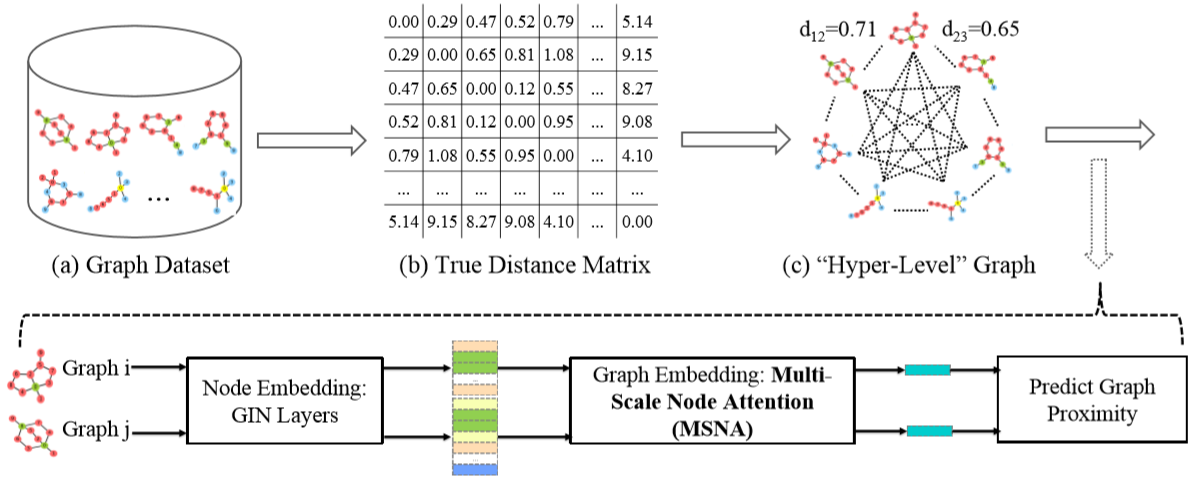
\includegraphics[width=.7\textwidth]{pics/UGraphEmb}
	\caption{Overview of UGraphEmb}
	\label{fig:UGraphEmb}
\end{figure}
% 接下来,构建一个Hyper-level graph --- 以图为结点,proximity作为边的权重。
\paragraph{UGraphEmb思路}首先,这个模型是在一个图数据集上学习的,需要先计算图数据集中两两图之间的proximity(一开始我认为是similarity,但并不是很准确,论文中使用的是GED来计算的proximity),这样就可以得到一个distance matrix,表示任意两个图之间的proximity。那么如何生成图的表征呢?使用GIN\cite{xu2018how}来学习结点表征,多尺度则体现在:以GIN的每一层生成一个图表征,再拼接在一起形成最终的图表征。其中每一层会有一个注意力,也就是MSNA。得到任意两个图的表征后,就要使用proximity了,希望模型学习到的图表征尽量保留图之间的proximity。损失函数定义如下:
% 公式换行!!!
% 其中 & 表示对齐的位置, \\ 表示换行
\begin{equation}\nonumber
	\begin{aligned}
		\mathcal{L} &= \mathbb{E}_{(i, j) \sim \mathcal{D}} (\hat{d_{ij} } - d_{ij} )\\
		&= \mathbb{E}_{(i, j) \sim \mathcal{D}} (||\boldsymbol{h_i} - \boldsymbol{h_j} ||_2^2 - d_{ij} )
	\end{aligned}
\end{equation}
其中$\hat{d_{ij} }$是关于两个图表征的proximity计算,$d_{ij}$是预先计算好的proximity。

论文中提到了\tbred{图表征的无监督学习方法的一个挑战}:与结点表征学习的不同,结点之间存在联系,可以在此基础上进行无监督学习,而图之间是没有天然的联系的(如距离/相似性)。而proximity就充当了一个这样的\textbf{Inter-Graph information},将不同的图联系起来。

\paragraph{方法解决的问题/优势}
\begin{itemize}
	\item 无监督的、inductive的图表征方法
	\item 可以作为图数据的预训练模型,下游任务在其基础上进行微调即可,如图分类、图相似性计算
\end{itemize}

\paragraph{方法的局限性/未来方向}
\begin{itemize}
	\item 能否直接在Hyper-level graph上学习图的表征与多尺度的表征融合呢?
%	\item 
\end{itemize}


